% Created by tikzDevice version 0.12.6 on 2025-12-23 06:16:01
% !TEX encoding = UTF-8 Unicode
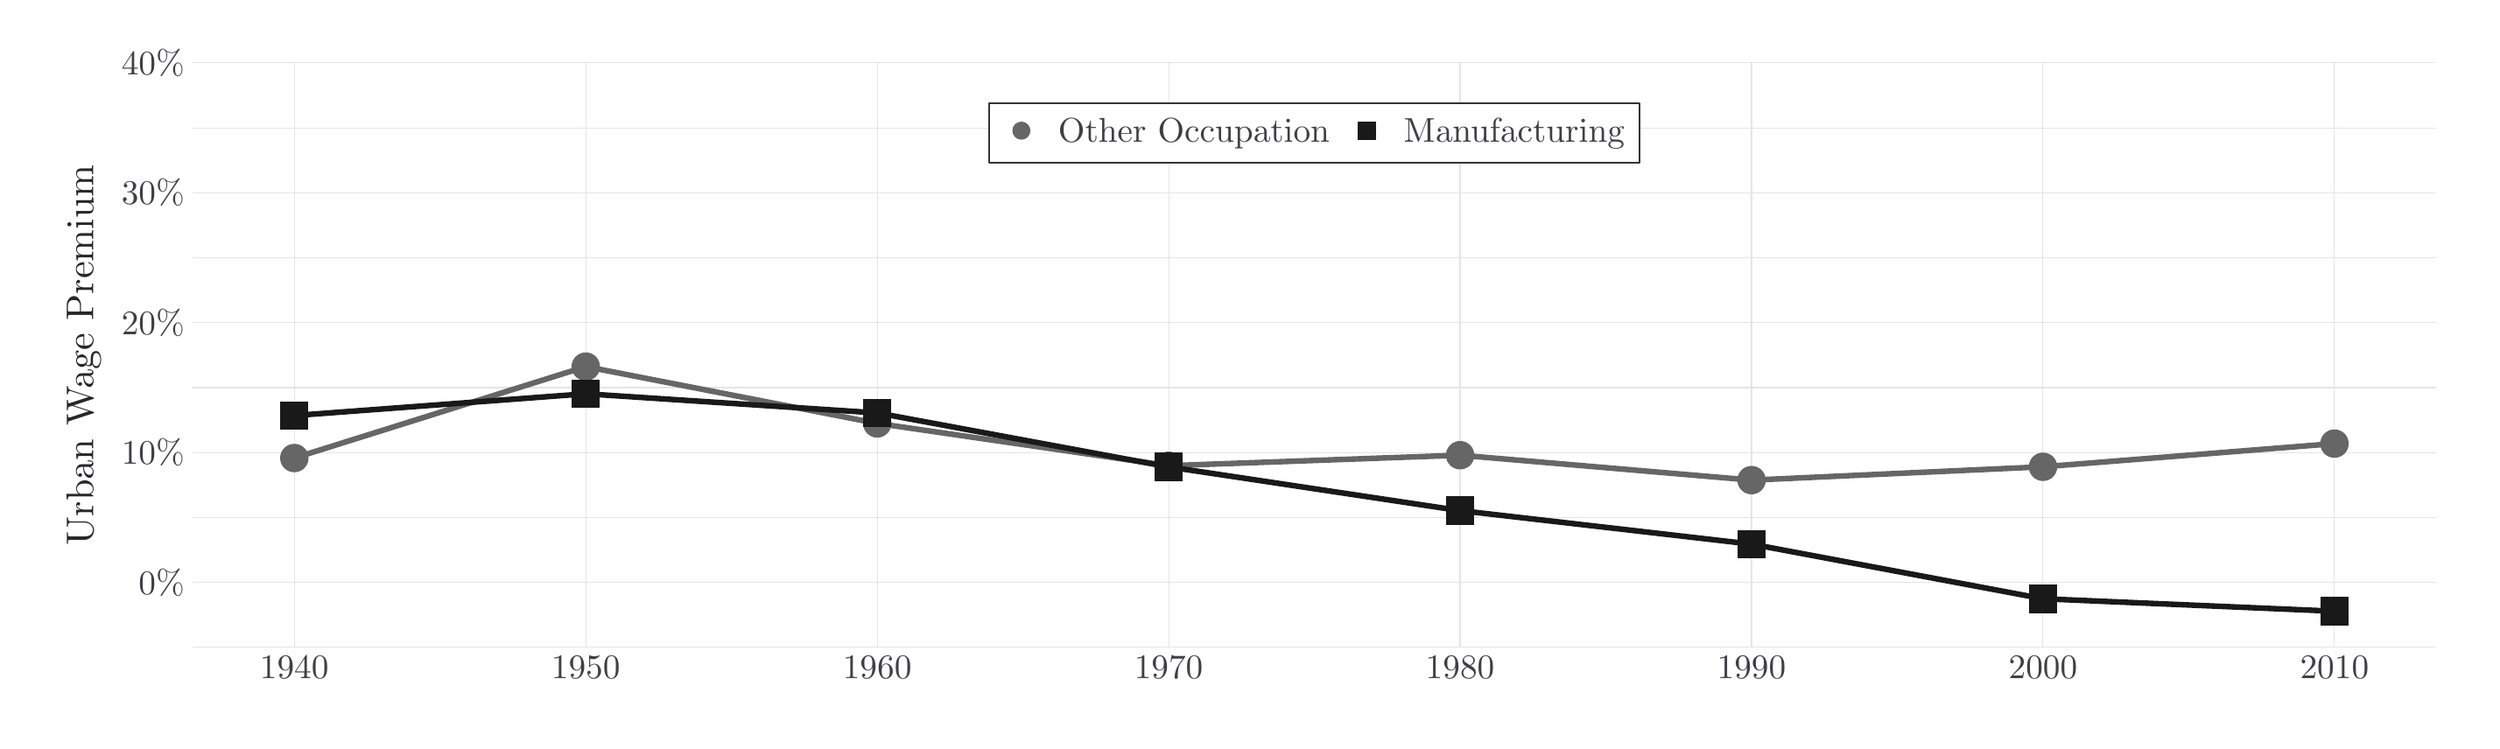
\begin{tikzpicture}[x=1pt,y=1pt]
\definecolor{fillColor}{RGB}{255,255,255}
\path[use as bounding box,fill=fillColor] (0,0) rectangle (1011.78,289.08);
\begin{scope}
\path[clip] (  0.00,  0.00) rectangle (1011.78,289.08);
\definecolor{drawColor}{RGB}{255,255,255}

\path[draw=drawColor,line width= 0.8pt,line join=round,line cap=round,fill=fillColor] (  0.00,  0.00) rectangle (1011.78,289.08);
\end{scope}
\begin{scope}
\path[clip] ( 69.39, 31.76) rectangle (995.78,273.08);
\definecolor{drawColor}{RGB}{255,255,255}
\definecolor{fillColor}{RGB}{255,255,255}

\path[draw=drawColor,line width= 0.8pt,line join=round,line cap=round,fill=fillColor] ( 69.39, 31.76) rectangle (995.78,273.08);
\definecolor{drawColor}{RGB}{228,228,231}

\path[draw=drawColor,line width= 0.4pt,line join=round] ( 69.39, 31.76) --
	(995.78, 31.76);

\path[draw=drawColor,line width= 0.4pt,line join=round] ( 69.39, 85.39) --
	(995.78, 85.39);

\path[draw=drawColor,line width= 0.4pt,line join=round] ( 69.39,139.01) --
	(995.78,139.01);

\path[draw=drawColor,line width= 0.4pt,line join=round] ( 69.39,192.64) --
	(995.78,192.64);

\path[draw=drawColor,line width= 0.4pt,line join=round] ( 69.39,246.27) --
	(995.78,246.27);

\path[draw=drawColor,line width= 0.4pt,line join=round] ( 69.39, 58.57) --
	(995.78, 58.57);

\path[draw=drawColor,line width= 0.4pt,line join=round] ( 69.39,112.20) --
	(995.78,112.20);

\path[draw=drawColor,line width= 0.4pt,line join=round] ( 69.39,165.83) --
	(995.78,165.83);

\path[draw=drawColor,line width= 0.4pt,line join=round] ( 69.39,219.45) --
	(995.78,219.45);

\path[draw=drawColor,line width= 0.4pt,line join=round] ( 69.39,273.08) --
	(995.78,273.08);

\path[draw=drawColor,line width= 0.4pt,line join=round] (111.50, 31.76) --
	(111.50,273.08);

\path[draw=drawColor,line width= 0.4pt,line join=round] (231.81, 31.76) --
	(231.81,273.08);

\path[draw=drawColor,line width= 0.4pt,line join=round] (352.12, 31.76) --
	(352.12,273.08);

\path[draw=drawColor,line width= 0.4pt,line join=round] (472.43, 31.76) --
	(472.43,273.08);

\path[draw=drawColor,line width= 0.4pt,line join=round] (592.74, 31.76) --
	(592.74,273.08);

\path[draw=drawColor,line width= 0.4pt,line join=round] (713.05, 31.76) --
	(713.05,273.08);

\path[draw=drawColor,line width= 0.4pt,line join=round] (833.36, 31.76) --
	(833.36,273.08);

\path[draw=drawColor,line width= 0.4pt,line join=round] (953.67, 31.76) --
	(953.67,273.08);
\definecolor{drawColor}{gray}{0.40}

\path[draw=drawColor,line width= 2.3pt,line join=round] (111.50,109.92) --
	(231.81,147.68) --
	(352.12,124.23) --
	(472.43,106.75) --
	(592.74,111.09) --
	(713.05,100.80) --
	(833.36,106.31) --
	(953.67,115.88);
\definecolor{drawColor}{gray}{0.10}

\path[draw=drawColor,line width= 2.3pt,line join=round] (111.50,127.47) --
	(231.81,136.45) --
	(352.12,128.55) --
	(472.43,106.26) --
	(592.74, 88.21) --
	(713.05, 74.37) --
	(833.36, 51.81) --
	(953.67, 46.66);
\definecolor{fillColor}{gray}{0.40}

\path[fill=fillColor] (111.50,109.92) circle (  5.87);
\definecolor{fillColor}{gray}{0.10}

\path[fill=fillColor] (105.63,121.60) --
	(117.37,121.60) --
	(117.37,133.34) --
	(105.63,133.34) --
	cycle;
\definecolor{fillColor}{gray}{0.40}

\path[fill=fillColor] (231.81,147.68) circle (  5.87);
\definecolor{fillColor}{gray}{0.10}

\path[fill=fillColor] (225.94,130.58) --
	(237.68,130.58) --
	(237.68,142.32) --
	(225.94,142.32) --
	cycle;
\definecolor{fillColor}{gray}{0.40}

\path[fill=fillColor] (352.12,124.23) circle (  5.87);
\definecolor{fillColor}{gray}{0.10}

\path[fill=fillColor] (346.25,122.68) --
	(357.99,122.68) --
	(357.99,134.42) --
	(346.25,134.42) --
	cycle;
\definecolor{fillColor}{gray}{0.40}

\path[fill=fillColor] (472.43,106.75) circle (  5.87);
\definecolor{fillColor}{gray}{0.10}

\path[fill=fillColor] (466.56,100.39) --
	(478.30,100.39) --
	(478.30,112.13) --
	(466.56,112.13) --
	cycle;
\definecolor{fillColor}{gray}{0.40}

\path[fill=fillColor] (592.74,111.09) circle (  5.87);
\definecolor{fillColor}{gray}{0.10}

\path[fill=fillColor] (586.87, 82.33) --
	(598.61, 82.33) --
	(598.61, 94.08) --
	(586.87, 94.08) --
	cycle;
\definecolor{fillColor}{gray}{0.40}

\path[fill=fillColor] (713.05,100.80) circle (  5.87);
\definecolor{fillColor}{gray}{0.10}

\path[fill=fillColor] (707.18, 68.50) --
	(718.92, 68.50) --
	(718.92, 80.24) --
	(707.18, 80.24) --
	cycle;
\definecolor{fillColor}{gray}{0.40}

\path[fill=fillColor] (833.36,106.31) circle (  5.87);
\definecolor{fillColor}{gray}{0.10}

\path[fill=fillColor] (827.49, 45.94) --
	(839.23, 45.94) --
	(839.23, 57.68) --
	(827.49, 57.68) --
	cycle;
\definecolor{fillColor}{gray}{0.40}

\path[fill=fillColor] (953.67,115.88) circle (  5.87);
\definecolor{fillColor}{gray}{0.10}

\path[fill=fillColor] (947.80, 40.79) --
	(959.54, 40.79) --
	(959.54, 52.53) --
	(947.80, 52.53) --
	cycle;
\end{scope}
\begin{scope}
\path[clip] (  0.00,  0.00) rectangle (1011.78,289.08);
\definecolor{drawColor}{RGB}{63,63,70}

\node[text=drawColor,anchor=base east,inner sep=0pt, outer sep=0pt, scale=  1.42] at ( 66.19, 53.67) {0\%};

\node[text=drawColor,anchor=base east,inner sep=0pt, outer sep=0pt, scale=  1.42] at ( 66.19,107.30) {10\%};

\node[text=drawColor,anchor=base east,inner sep=0pt, outer sep=0pt, scale=  1.42] at ( 66.19,160.93) {20\%};

\node[text=drawColor,anchor=base east,inner sep=0pt, outer sep=0pt, scale=  1.42] at ( 66.19,214.56) {30\%};

\node[text=drawColor,anchor=base east,inner sep=0pt, outer sep=0pt, scale=  1.42] at ( 66.19,268.18) {40\%};
\end{scope}
\begin{scope}
\path[clip] (  0.00,  0.00) rectangle (1011.78,289.08);
\definecolor{drawColor}{RGB}{63,63,70}

\node[text=drawColor,anchor=base,inner sep=0pt, outer sep=0pt, scale=  1.42] at (111.50, 18.76) {1940};

\node[text=drawColor,anchor=base,inner sep=0pt, outer sep=0pt, scale=  1.42] at (231.81, 18.76) {1950};

\node[text=drawColor,anchor=base,inner sep=0pt, outer sep=0pt, scale=  1.42] at (352.12, 18.76) {1960};

\node[text=drawColor,anchor=base,inner sep=0pt, outer sep=0pt, scale=  1.42] at (472.43, 18.76) {1970};

\node[text=drawColor,anchor=base,inner sep=0pt, outer sep=0pt, scale=  1.42] at (592.74, 18.76) {1980};

\node[text=drawColor,anchor=base,inner sep=0pt, outer sep=0pt, scale=  1.42] at (713.05, 18.76) {1990};

\node[text=drawColor,anchor=base,inner sep=0pt, outer sep=0pt, scale=  1.42] at (833.36, 18.76) {2000};

\node[text=drawColor,anchor=base,inner sep=0pt, outer sep=0pt, scale=  1.42] at (953.67, 18.76) {2010};
\end{scope}
\begin{scope}
\path[clip] (  0.00,  0.00) rectangle (1011.78,289.08);
\definecolor{drawColor}{RGB}{39,39,42}

\node[text=drawColor,rotate= 90.00,anchor=base,inner sep=0pt, outer sep=0pt, scale=  1.60] at ( 28.57,152.42) {Urban Wage Premium};
\end{scope}
\begin{scope}
\path[clip] (  0.00,  0.00) rectangle (1011.78,289.08);
\definecolor{drawColor}{gray}{0.20}
\definecolor{fillColor}{RGB}{255,255,255}

\path[draw=drawColor,line width= 0.8pt,line join=round,line cap=round,fill=fillColor] (398.41,231.89) rectangle (666.77,256.35);
\end{scope}
\begin{scope}
\path[clip] (  0.00,  0.00) rectangle (1011.78,289.08);
\definecolor{drawColor}{RGB}{255,255,255}
\definecolor{fillColor}{RGB}{255,255,255}

\path[draw=drawColor,line width= 0.8pt,line join=round,line cap=round,fill=fillColor] (404.41,237.89) rectangle (418.86,252.35);

\path[] (405.85,245.12) -- (417.41,245.12);
\definecolor{fillColor}{gray}{0.40}

\path[fill=fillColor] (411.63,245.12) circle (  3.73);
\end{scope}
\begin{scope}
\path[clip] (  0.00,  0.00) rectangle (1011.78,289.08);
\definecolor{drawColor}{RGB}{255,255,255}
\definecolor{fillColor}{RGB}{255,255,255}

\path[draw=drawColor,line width= 0.8pt,line join=round,line cap=round,fill=fillColor] (547.05,237.89) rectangle (561.51,252.35);

\path[] (548.50,245.12) -- (560.06,245.12);
\definecolor{fillColor}{gray}{0.10}

\path[fill=fillColor] (550.55,241.39) --
	(558.01,241.39) --
	(558.01,248.85) --
	(550.55,248.85) --
	cycle;
\end{scope}
\begin{scope}
\path[clip] (  0.00,  0.00) rectangle (1011.78,289.08);
\definecolor{drawColor}{RGB}{63,63,70}

\node[text=drawColor,anchor=base west,inner sep=0pt, outer sep=0pt, scale=  1.42] at (426.86,240.22) {Other Occupation};
\end{scope}
\begin{scope}
\path[clip] (  0.00,  0.00) rectangle (1011.78,289.08);
\definecolor{drawColor}{RGB}{63,63,70}

\node[text=drawColor,anchor=base west,inner sep=0pt, outer sep=0pt, scale=  1.42] at (569.51,240.22) {Manufacturing};
\end{scope}
\end{tikzpicture}
